% Copyright 2018-2020 Melvin Eloy Irizarry-Gelpí
\setcounter{chapter}{5}
\chapter{RLC Circuits}
%
In this experiment you will study circuits with resistors, inductors, and capacitors interacting with a source of alternating currents.
%
\section{Preliminary}
%
In a previous experiment, you studied RC and RL circuits with a \textbf{battery} (actually, a few batteries connected in series) as the source of current. Batteries provide \textbf{DC} or \textbf{direct currents}, meaning that over time the current does not change direction. Strictly speaking the previous circuits were DC circuits.

When the current switches direction over time, you have an \textbf{AC} or \textbf{alternating current}. A circuit with an AC source is called an \textbf{AC circuit}. An important parameter that describes how often an AC switches direction is $f$, the \textbf{frequency of oscillation}. Recall that frequency is a quantity measured in \textbf{hertz} (Hz). One hertz is equivalent to one full oscillation per second:
\begin{equation}
	1 \ \text{Hz} = 1 \ \text{oscillation/s}
\end{equation}
For an AC with a frequency of 1 Hz, this means that it takes 1 second for the current to do a full oscillation. Note that a full current oscillation involves two switches of current direction: the first switch changes the original direction and the second switch returns it to where it was originally. Another useful quantity is $T$, the \textbf{period of oscillation}. The period $T$ is related to the frequency $f$ via
\begin{equation} \label{eq.06.period}
	T = \frac{1}{f}
\end{equation}
Sometimes it will be useful to use frequency and sometimes it will be useful to use period.

A quick reminder that electrical \textbf{resistance} is measured in units of ohms;
\begin{equation}
	1 \ \text{ohm} = 1 \ \text{V/A}
\end{equation}
\textbf{capacitance} is measured in units of farads;
\begin{equation}
	1 \ \text{farad} = 1 \ \text{C/V} = 1 \ \text{s/ohm}
\end{equation}
and \textbf{inductance} is measured in units of henrys;
\begin{equation}
	1 \ \text{henry} = 1 \ \text{V{ }\textperiodcentered{ }s/A} = 1 \ \text{ohm{ }\textperiodcentered{ }s}
\end{equation}
%
\subsection{Reactance}
%
Resistors, capacitors and inductors behave differently in an AC circuit. Each of these components display an opposition to the change in electric current that is called \textbf{reactance}. The mathematical symbol for reactance is $X$. There is \textbf{resistive} reactance $X_{R}$, \textbf{capacitive} reactance $X_{C}$, and \textbf{inductive} reactance $X_{L}$. Each reactance quantity is measured in units of ohms (same as resistance).
%
\subsubsection{Resistive Reactance}
%
The reactance associated to a resistor is called resistive reactance. For all practical purposes, the \textbf{resistive reactance} $X_{R}$ of a given resistor is equal to the resistance $R$:
\begin{equation} \label{eq.06.reactance.R}
	X_{R} = R
\end{equation}
Note that $X_{R}$ only depends on the properties of the resistor and not on the frequency of the AC source. That is, it does not matter how often the current switches direction, the resistive reactance is the same.
%
\subsubsection{Capacitive Reactance}
%
The reactance associated to a capacitor is called capacitive reactance. The \textbf{capacitive reactance} $X_{C}$ of a given capacitor is given by
\begin{equation} \label{eq.06.reactance.C}
	X_{C} = \frac{1}{2 \pi f C} = \frac{T}{2 \pi C}
\end{equation}
Here $f$ is the frequency of oscillation of the AC source, $T$ is the period of oscillation of the AC source, and $C$ is the amount of capacitance in the capacitor. Note that $X_{C}$ is directly proportional to the period, or, equivalently, inversely proportional to the frequency. That is, if you increase the frequency of the AC source, then the reactance should decrease.
%
\subsubsection{Inductive Reactance}
%
The reactance associated to an inductor is called inductive reactance. The \textbf{inductive reactance} $X_{L}$ of a given inductor is defined as
\begin{equation} \label{eq.06.reactance.L}
	X_{L} = 2 \pi f L = \frac{2 \pi L}{T}
\end{equation}
Here $f$ is the frequency of oscillation of the AC source, $T$ is the period of oscillation of the AC source, and $L$ is the amount of inductance in the inductor. Note that $X_{L}$ is directly proportional to the frequency, or, equivalently, inversely proportional to the period. That is, if you increase the frequency of the AC source, then the reactance should increase.
%
\subsection{Impedance}
%
Reactance is associated with an individual component in a circuit. To describe the \textbf{entire circuit}, you use the \textbf{impedance} $Z$. Just like reactance and resistance, impedance is also measured in units of ohms. The exact definition of impedance depends on what the components in a circuit are. You are going to need the impedance for an RL and RLC circuit.
%
\subsubsection{RL AC Circuit}
%
An \textbf{RL AC circuit} consist of an \textbf{AC source} connected to a \textbf{resistor} and an \textbf{ideal inductor} in series. Thus there is some amount of resistive and inductive reactance. The RL impedance $Z$ takes these two contributions into account:
\begin{equation} \label{eq.06.impedance.RL}
	Z = \sqrt{X_{R}^{2} + X_{L}^{2}} = \sqrt{R^{2} + 4 \pi^{2} f^{2} L^{2}}
\end{equation}
You can think of $Z$ as the hypotenuse of a right triangle with the reactances $X_{R}$ and $X_{L}$ as sides. The squared impedance takes the form
\begin{equation} \label{eq.06.impedance.squared}
	Z^{2} = R^{2} + 4\pi^{2} f^{2} L^{2}
\end{equation}
Note that in this form, the relation between squared impedance and squared frequency lends itself for a linear fit: the intercept is the squared resistance, and the slope is proportional to the squared inductance.

An ideal inductor has negligible electrical resistance. In practice you work with \textbf{non-ideal inductors}, with a non-negligible amount of electrical resistance $r$. This can be taken into account as follows:
\begin{equation}
	Z^{2} = (R + r)^{2} + 4 \pi^{2} f^{2} L^{2}
\end{equation}
That is, the resistance from the inductor affects the value of the intercept of the linear fit.
%
\subsubsection{RLC AC Circuit}
%
An \textbf{RLC AC circuit} consist of an \textbf{AC source} connected to a \textbf{resistor}, a \textbf{capacitor}, and an \textbf{ideal inductor} in series. Now there is some amount of resistive, capacitive, and inductive reactance. The RLC impedance $Z$ now takes these three contributions into account:
\begin{equation} \label{eq.06.eq.06.impedance.RLC}
	Z = \sqrt{X_{R}^{2} + X_{L}^{2} - X_{C}^{2}} = \sqrt{R^{2} + 4 \pi^{2} f^{2} L^{2} - \frac{1}{4 \pi^{2} f^{2} C^{2}}}
\end{equation}
Something special happens when $X_{L} = X_{C}$:
\begin{align} \label{eq.06.resonant.frequency}
	X_{L}(f_{\text{LC}}) = X_{C}(f_{\text{LC}}) && \Longrightarrow && 2\pi f_{\text{LC}} L = \frac{1}{2\pi f_{\text{LC}} C} && \Longrightarrow && f_{\text{LC}} = \frac{1}{2 \pi \sqrt{LC}}
\end{align}
That is, when the frequency takes the special value $f_{\text{LC}}$ (that depends on the amount of inductance and capacitance), the impedance is given entirely by the amount of resistance. This situation is called \textbf{resonance} and $f_{\text{LC}}$ is known as the \textbf{resonant frequency}. When the values of the capacitance and inductance in the circuit conspire to achieve the resonant frequency, the impedance reduces to the resistance:
\begin{equation}
	Z = R
\end{equation}
This is the minimum value possible of impedance.
%
\section{Experiment}
%
There are four experiments:
\begin{enumerate}
	\item Capacitor in AC circuit
	\item RL AC circuit
	\item RLC AC circuit without the core
	\item RLC AC circuit with the core
\end{enumerate}
In the first two experiments you measure the voltage and current as the frequency of the AC is changed. In the last two experiments, you see the effects of the resonance state.
%
\subsection{Part 1: Capacitor AC Circuit}
%
The circuit has \textbf{one capacitor} (10\textsuperscript{\textminus 5} F) connected to an AC source whose frequency you can adjust. You measured voltage and current over time. For each measurement you change the frequency of the AC source. The range of frequencies is from 100 Hz to 1000 Hz. Table \ref{table.capacitor.student} has the frequency values used for each run.

Note that the voltage measured here is the \textbf{voltage across the capacitor}.
%
\subsection{Part 2: RL AC Circuit}
%
The circuit has \textbf{one resistor} (10 ohm) and \textbf{one non-ideal inductor} (0.005 H and 4.20 ohm) connected in series to an AC source whose frequency you can adjust. You measured voltage and current over time. For each measurement you change the frequency of the AC source. The range of frequencies is from 100 Hz to 1000 Hz. Table \ref{table.RL.student} has the frequency values used for each run.

Note that the voltage measured here is the \textbf{voltage across the resistor and inductor in series}. That is, between the input terminal of the resistor, and the output terminal of the inductor.
%
\subsection{Part 3: RLC AC Circuit (without core)}
%
The circuit has \textbf{one resistor} (in the form of a light bulb, with unknown resistance), \textbf{one capacitor} (10\textsuperscript{\textminus 5} F), and \textbf{one non-ideal inductor} (0.005 H and 4.20 ohm; without core) connected in series to an AC source whose frequency you can adjust. You measured current over time. For each measurement you change the frequency of the AC source. The range of frequencies is from 100 Hz to 1300 Hz. Table \ref{table.RLC.student} has the frequency values used for each run.
%
\subsection{Part 4: RLC AC Circuit (with core)}
%
The circuit has \textbf{one resistor} (in the form of a light bulb, with unknown resistance), \textbf{one capacitor} (10\textsuperscript{\textminus 5} F), and \textbf{one non-ideal inductor} (0.0213 H and 4.20 ohm; with core) connected in series to an AC source whose frequency you can adjust. You measured current over time. For each measurement you change the frequency of the AC source. The range of frequencies is from 100 Hz to 550 Hz. Table \ref{table.RLCcore.student} has the frequency values used for each run.
%
\section{Analysis}
%
Here is what to do for each part.
%
\subsection{Part 1: Capacitor AC Circuit}
%
The impedance of a circuit with a single capacitor is just the capacitive reactance:
\begin{equation}
	Z = X_{C} = \left(\frac{1}{2 \pi C}\right) \frac{1}{f} = \left(\frac{1}{2 \pi C}\right) T
\end{equation}
In this part you would like to check that the inductance is inversely proportional to the frequency of the AC source, or equivalently, directly proportional to the period of the AC source. You know the values of the frequencies used (and thus of the periods used), so you just need to find the experimental values of $Z$. To find this, you use the voltage and current data. For each run, you find the maximum voltage $V_{\text{max}}$ and the maximum current in $I_{\text{max}}$. Then, the impedance is given by the ratio
\begin{equation}
	Z = \frac{V_{\text{max}}}{I_{\text{max}}}
\end{equation}
Once you have the impedance, you can check that the chart of impedance versus frequency is not linear, but the chart of impedance versus period is linear. You can then add a linear fit. As stated by (\ref{eq.06.reactance.C}), the slope is related to the amount of capacitance:
\begin{equation}
	\text{slope} = \frac{1}{2 \pi C}
\end{equation}
You can calculate the expected slope, the observed slope (use the \texttt{SLOPE}) function, and then calculate the percent difference:
\begin{equation}
	\text{Percent Difference} = 100 \times \left( \frac{\text{observed } - \text{ expected}}{\text{expected}} \right)
\end{equation}
%
\subsection{Part 2: RL AC Circuit}
%
Since an RL AC circuit is used in this part, you can check the relationship between impedance $Z$ and frequency (that is, you are not measuring the reactance of individual components). The impedance is found in the same way as before:
\begin{equation}
	Z = \frac{V_{\text{max}}}{I_{\text{max}}}
\end{equation}
You can chart impedance versus frequency and the shape is almost linear. But there is no linear relationship between these two quantities! Looking at (\ref{eq.06.impedance.squared}), the expected linear relationship is between $Z^{2}$ and $f^{2}$. Make a second chart with these quantities and add a best-fit line. Compare the slope and intercept of the best-fit line to the expected values in (\ref{eq.06.impedance.squared}). The slope should be related to the inductance, and the intercept should be related to the \textbf{total amount of resistance} in the circuit. Recall that the inductor has some inherent amount of resistance, as was found in Laboratory 5:
\begin{equation}
	r = 4.20 \ \text{ohm}
\end{equation}
Adding this to the 10 ohm from the resistor, the total resistance is
\begin{equation}
	R_{\text{eq}} = R + r = 14.20 \ \text{ohm}
\end{equation}
The expected slope is
\begin{equation}
	\text{slope} = 4 \pi^{2} L^{2}
\end{equation}
and the expected intercept is
\begin{equation}
	\text{intercept} = (R + r)^{2}
\end{equation}
Again, you can also find the percent difference to judge the quality of your results.
%
\subsection{Part 3: RLC AC Circuit (without core)}
%
For the RLC circuit, you can see what happens to the current in the circuit as the frequency of the AC source  approaches the value of the resonant frequency. To do this, find the maximum current for each frequency run and then make a chart of $I_{\text{max}}$ versus frequency. There should be a peak. The peak corresponds to the resonant frequency. That is, at the resonant frequency, the current in the circuit oscillates with the largest amplitude.

The expected resonant frequency is given by (\ref{eq.06.resonant.frequency}), with the inductance equal to 0.005 H.
%
\subsection{Part 4: RLC AC Circuit (with core)}
%
In Laboratory 5 you found that when the core was used, the inductance is larger than what is written on the label. Indeed, you should have found a value close to 0.0213 H. This makes the resonant frequency smaller. You can repeat the steps as in Part 3 and confirm that the current now has a peak in a lower frequency.
%
\section{My Data}
%
My results for Part 1 are in Table \ref{table.results.C}. As you can see from Figure \ref{figure.06.part.1.f}, in this circuit the impedance is not directly proportional to the frequency. Indeed, as you can see from Figure \ref{figure.06.part.1.T}, the impedance is directly proportional to the period of oscillation. The result is that as the frequency is increased, the impedance decreases, and thus the amount of current allowed increases.

My results for Part 2 are in Table \ref{table.results.RL}. Figure \ref{figure.06.part.2.f} appears to indicate that the impedance is directly proportional to the amount of frequency. However, the best fit is off for some values. Looking at the squared impedance versus the squared frequency in Figure \ref{figure.06.part.2.f2} shows that the linear relation is stronger between those two quantities. Opposite to what happens in Part 1, when the frequency is increased, the impedance also increases, and thus the amount of current allowed decreases.

My results for Part 3 are in Table \ref{table.results.RLC}. As you can see from Figure \ref{figure.06.part.3.f}, the current is largest in a certain region consistent with the theoretical expectation. Note that when the current is largest, the impedance is smallest.

My results for Part 4 are in Table \ref{table.results.RLCcore}. When the core is used, the inductance becomes larger. This should have the effect of making the resonant frequency smaller. As Figure \ref{figure.06.part.4.f} shows, this is indeed the case.
%
\section{Your Data}
%
Your data for Parts 1, 2, 3, and 4 is structured in the same way as Tables \ref{table.capacitor.student}, \ref{table.RL.student}, \ref{table.RLC.student}, and \ref{table.RLCcore.student}.
%
\pagebreak
\section{Your Lab Report}
%
Your laboratory report should include the following:
\begin{itemize}
	\item A table like Table \ref{table.results.C} with your results for part 1.
	\item A chart like Figure \ref{figure.06.part.1.T} with impedance in the vertical axis, and period in the horizontal axis for the data in part 1. Include the best fit line and display the equation.
	\item A table like Table \ref{table.results.RL} with your results for part 2.
	\item A chart like Figure \ref{figure.06.part.2.f2} with squared impedance in the vertical axis, and squared frequency in the horizontal axis for the data in part 2. Include the best fit line and display the equation.
	\item A chart like Figure \ref{figure.06.part.3.f} with maximum current in the vertical axis, and frequency in the horizontal axis for the data in part 3. Confirm that the maximum current corresponds occurs near frequencies that are close to the expected resonant frequency.
	\item A chart like Figure \ref{figure.06.part.4.f} with maximum current in the vertical axis, and frequency in the horizontal axis for the data in part 4. Confirm that the maximum current corresponds occurs near frequencies that are close to the expected resonant frequency.
\end{itemize}
%
\newpage
\section{Tables}
%
\begin{table}[ht]
	\begin{center}
		\begin{tabular}{l|r|r|r|r|r}
			\textbf{Run} & $f$ (Hz) & $1/f$ (s) & $V_{\text{max}}$ (V) & $I_{\text{max}}$ (A) & $V_{\text{max}}/I_{\text{max}}$ (ohm) \\
			\hline
			1 & 100 & & & & \\
			2 & 250 & & & & \\
			3 & 400 & & & & \\
			4 & 550 & & & & \\
			5 & 700 & & & & \\
			6 & 850 & & & & \\
			7 & 1000 & & & & \\
			\hline
		\end{tabular}
	\end{center}
	\caption{Capacitor AC Circuit}
	\label{table.capacitor.student}
\end{table}
%
\begin{table}[ht]
	\begin{center}
		\begin{tabular}{l|r|r|r|r|r}
			\textbf{Run} & $f$ (Hz) & $1/f$ (s) & $V_{\text{max}}$ (V) & $I_{\text{max}}$ (A) & $V_{\text{max}}/I_{\text{max}}$ (ohm) \\
			\hline
			1 & 100 & & & & \\
			2 & 250 & & & & \\
			3 & 400 & & & & \\
			4 & 550 & & & & \\
			5 & 700 & & & & \\
			6 & 850 & & & & \\
			7 & 1000 & & & & \\
			\hline
		\end{tabular}
	\end{center}
	\caption{RL AC Circuit}
	\label{table.RL.student}
\end{table}
%
\begin{table}[ht]
	\begin{center}
		\begin{tabular}{l|r|r}
			\textbf{Run} & $f$ (Hz) & $I_{\text{max}}$ (A) \\
			\hline
			1 & 100 & \\
			2 & 250 & \\
			3 & 400 & \\
			4 & 550 & \\
			5 & 700 & \\
			6 & 850 & \\
			7 & 1000 & \\
			8 & 1150 & \\
			9 & 1300 & \\
			\hline
		\end{tabular}
	\end{center}
	\caption{RLC AC Circuit without core}
	\label{table.RLC.student}
\end{table}
%
\begin{table}[ht]
	\begin{center}
		\begin{tabular}{l|r|r}
			\textbf{Run} & $f$ (Hz) & $I_{\text{max}}$ (A) \\
			\hline
			1 & 100 & \\
			2 & 250 & \\
			3 & 400 & \\
			4 & 550 & \\
			5 & 200 & \\
			6 & 300 & \\
			7 & 350 & \\
			8 & 450 & \\
			9 & 500 & \\
			\hline
		\end{tabular}
	\end{center}
	\caption{RLC AC Circuit with core}
	\label{table.RLCcore.student}
\end{table}
%
\begin{table}[ht]
	\begin{center}
		\begin{tabular}{l|r|r|r}
			\textbf{Quantity} & \textbf{Observed} & \textbf{Expected} & \textbf{P.D.} (\%) \\
			\hline
			Slope (ohm/s) & 14683.346 & 15915.494 & \textminus 7.742 \\
			\hline
		\end{tabular}
	\end{center}
	\caption{Results for capacitor AC circuit}
	\label{table.results.C}
\end{table}
%
\begin{table}[ht]
	\begin{center}
		\begin{tabular}{l|r|r|r}
			\textbf{Quantity} & \textbf{Observed} & \textbf{Expected} & \textbf{P.D.} (\%) \\
			\hline
			Slope (ohm\textsuperscript{2}/Hz\textsuperscript{2}) & 9.87{ }\texttimes{ }10\textsuperscript{\textminus 4} & 9.92{ }\texttimes{ }10\textsuperscript{\textminus 4} & 0.52 \\
			Intercept (ohm\textsuperscript{2}) & 199.778 & 201.64 & \textminus 0.924 \\
			\hline
		\end{tabular}
	\end{center}
	\caption{Results for RL AC circuit}
	\label{table.results.RL}
\end{table}
%
\begin{table}[ht]
	\begin{center}
		\begin{tabular}{l|r}
			Observed Resonant Frequency & Expected Resonant Frequency \\
			\hline
			Between 700 Hz and 800 Hz & 711.76 Hz \\
			\hline
		\end{tabular}
	\end{center}
	\caption{Results for RLC AC circuit (without core)}
	\label{table.results.RLC}
\end{table}
%
\begin{table}[ht]
	\begin{center}
		\begin{tabular}{l|r}
			Observed Resonant Frequency & Expected Resonant Frequency \\
			\hline
			Between 300 Hz and 350 Hz & 344.85 Hz \\
			\hline
		\end{tabular}
	\end{center}
	\caption{Results for RLC AC circuit (with core)}
	\label{table.results.RLCcore}
\end{table}
%
\newpage
\FloatBarrier
\section{Figures}
%
\begin{figure}[ht]
	\centering
	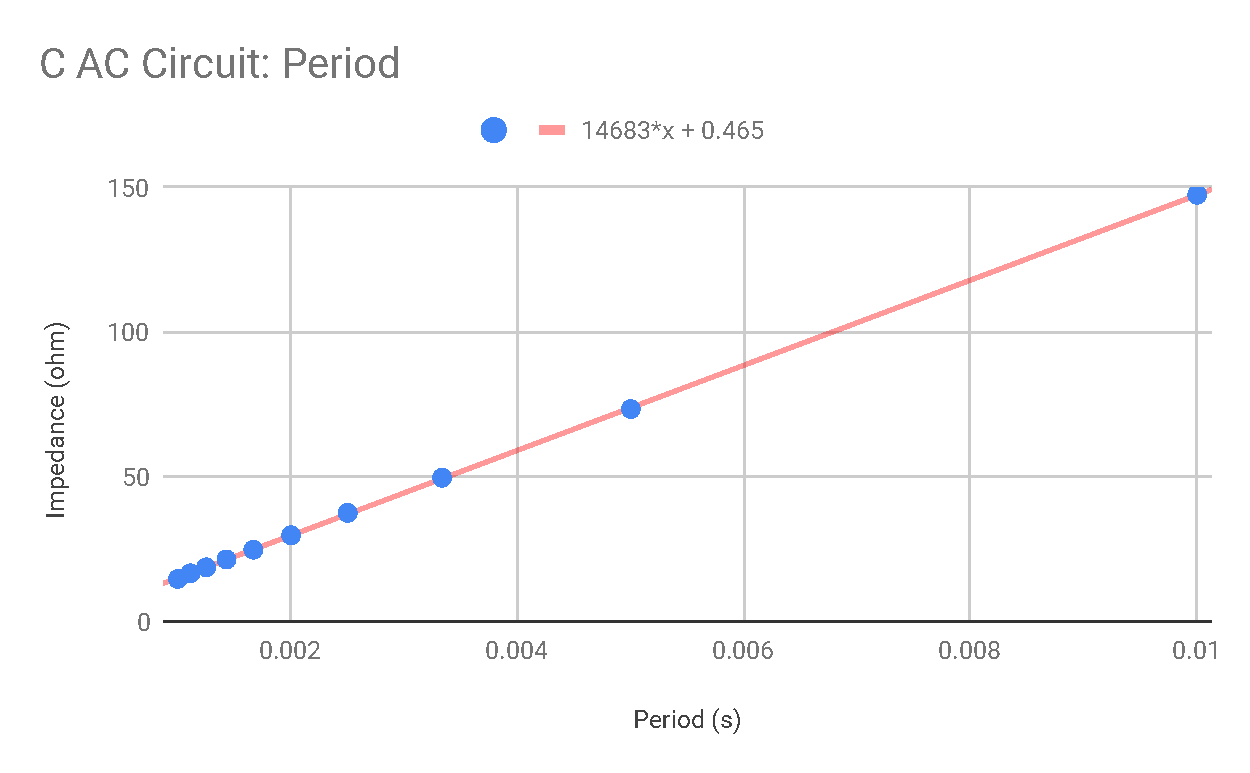
\includegraphics[scale=0.74]{image/06-RLC/part-1-f.pdf}
	\caption{Part 1: Period}
	\label{figure.06.part.1.f}
\end{figure}
%
\begin{figure}[ht]
	\centering
	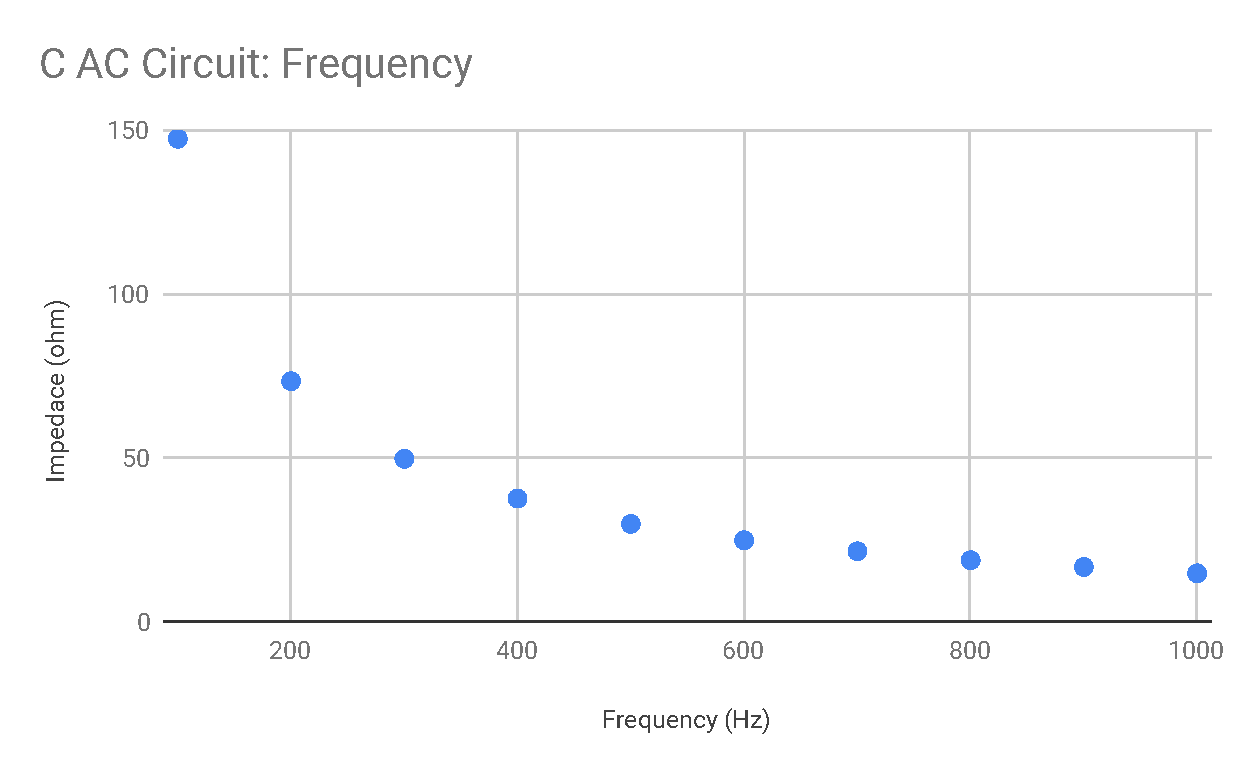
\includegraphics[scale=0.74]{image/06-RLC/part-1-T.pdf}
	\caption{Part 1: Frequency}
	\label{figure.06.part.1.T}
\end{figure}
%
\begin{figure}[ht]
	\centering
	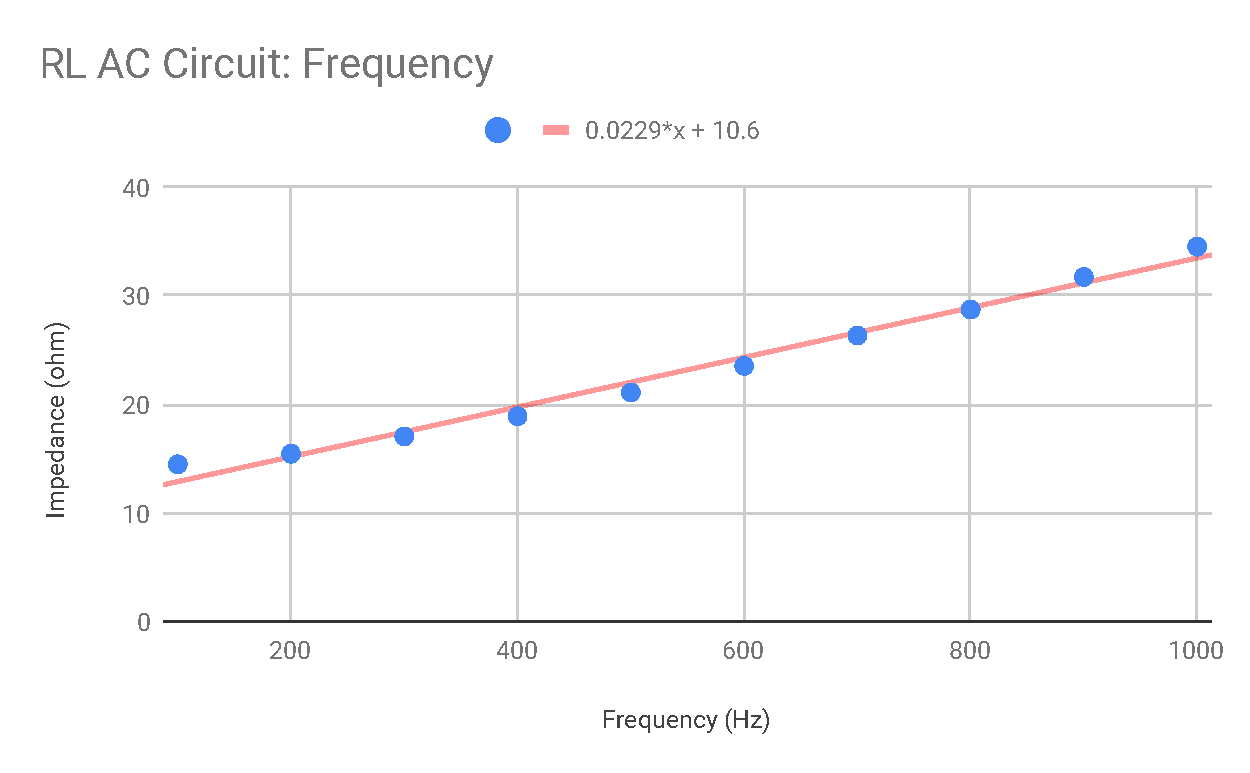
\includegraphics[scale=0.74]{image/06-RLC/part-2-f.pdf}
	\caption{Part 2: Frequency}
	\label{figure.06.part.2.f}
\end{figure}
%
\begin{figure}[ht]
	\centering
	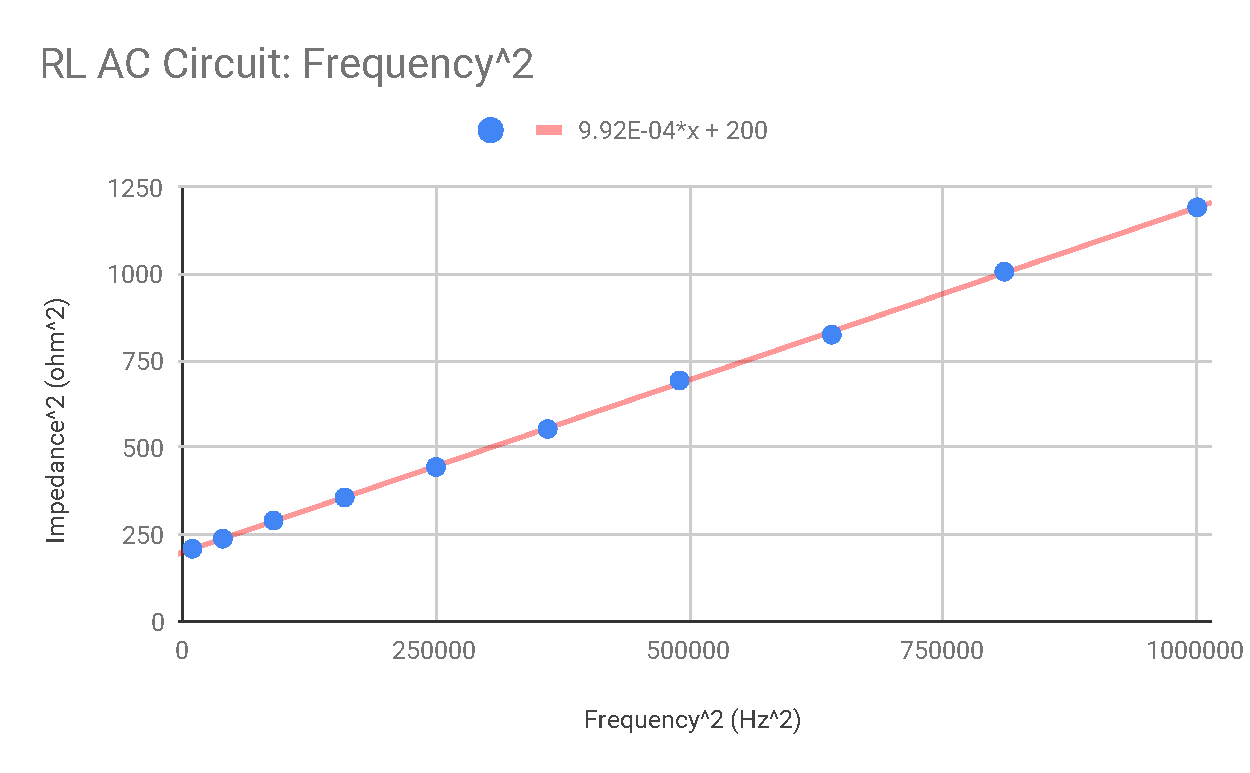
\includegraphics[scale=0.74]{image/06-RLC/part-2-f2.pdf}
	\caption{Part 2: Squared Frequency}
	\label{figure.06.part.2.f2}
\end{figure}
%
\begin{figure}[ht]
	\centering
	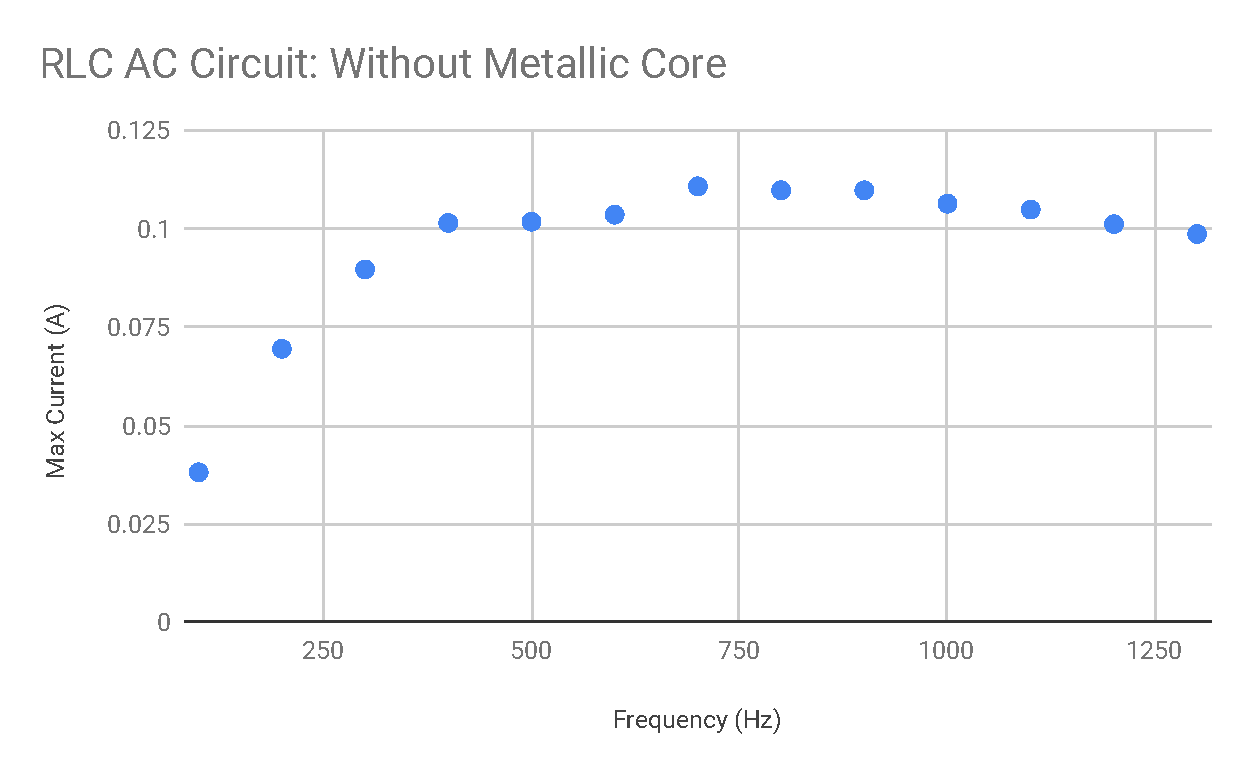
\includegraphics[scale=0.74]{image/06-RLC/part-3.pdf}
	\caption{Part 3}
	\label{figure.06.part.3.f}
\end{figure}
%
\begin{figure}[ht]
	\centering
	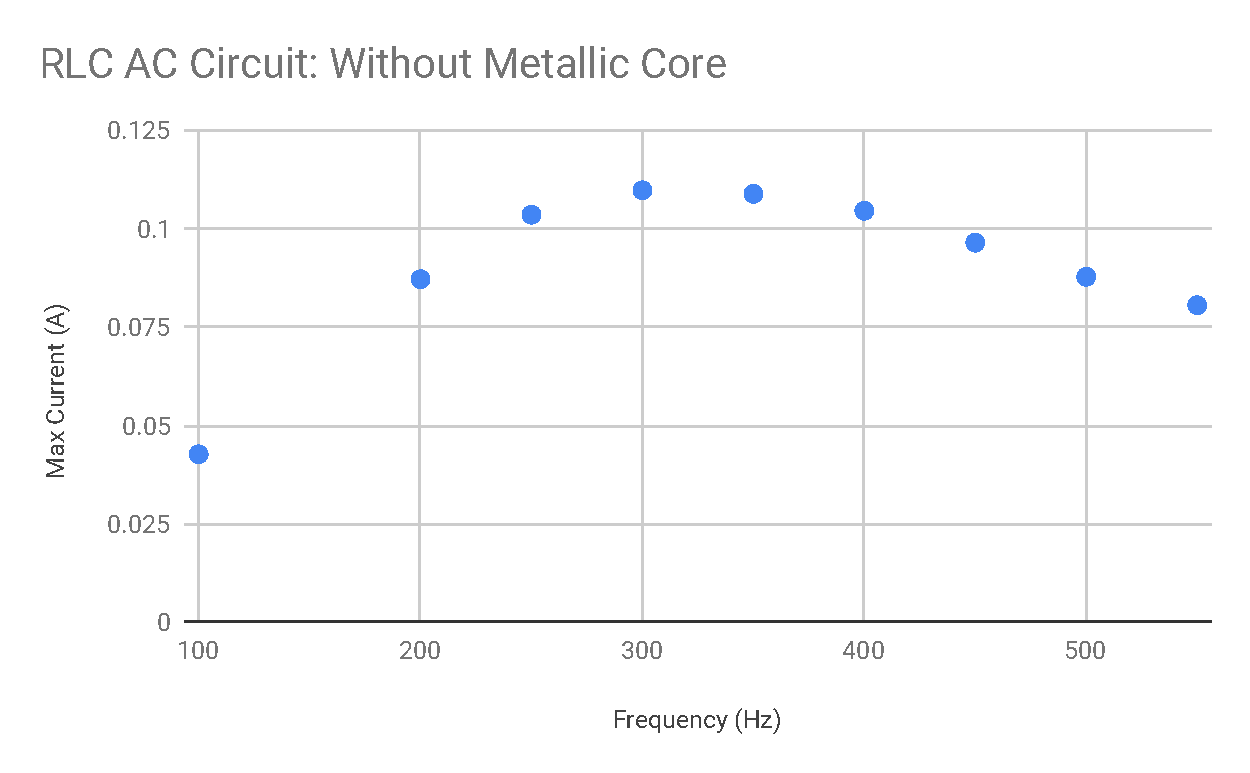
\includegraphics[scale=0.74]{image/06-RLC/part-4.pdf}
	\caption{Part 4}
	\label{figure.06.part.4.f}
\end{figure}
%